\documentclass[12pt]{article}
\usepackage[utf8]{inputenc}
\usepackage[a4paper, margin=2cm]{geometry}
\usepackage[T1]{fontenc}
\usepackage{graphicx}
\usepackage{geometry}
\usepackage{amsmath}
\usepackage{amsfonts}
\usepackage{amssymb}
\usepackage{booktabs}
\usepackage{hyperref}
\usepackage{fancyhdr}
\usepackage{float}
\usepackage{ulem}
\usepackage{xeCJK}
\usepackage{listings}
\usepackage{xcolor}
\usepackage{indentfirst}
\setmainfont{Times New Roman}
\setCJKmonofont[BoldFont=SimHei, AutoFakeBold=true]{SimSun}
\lstset{
    basicstyle=\ttfamily\small,
    commentstyle=\color{gray},
    keywordstyle=\color{blue},
    stringstyle=\color{red},
    numberstyle=\tiny\color{gray},
    breaklines=true,
    captionpos=b,
    keepspaces=true,
    numbers=left,
    numbersep=5pt,
    showspaces=false,
    showstringspaces=false,
    showtabs=false,
    tabsize=2,
    frame=single,
    language=[x86masm]Assembler
}

\begin{document}
\thispagestyle{empty}

\begin{center}
    \vspace*{2cm}
    
    \Huge \textbf{2023-2024学年春季学期} \\
    \vspace{2cm}
    
    \Huge \textbf{《汇编语言程序设计》} \\
    \vspace{4cm}
    
    \large 评分：\underline{\hspace{4cm}} \\
    \vspace{6cm}
    
    \begin{tabular}{rl}
        \Large 学\hspace{2em}院： & \Large \underline{\makebox[12em][l]{\quad 计算机科学与工程学院}} \\
        \Large 专\hspace{2em}业： & \Large \underline{\makebox[12em][l]{\quad 计算机科学与技术}} \\
        \Large 班\hspace{2em}级： & \Large \underline{\makebox[12em][l]{\quad 计算机2204班}} \\
        \Large 姓\hspace{2em}名： & \Large \underline{\makebox[12em][l]{\quad 李俊洁}} \\
        \Large 学\hspace{2em}号： & \Large \underline{\makebox[12em][l]{\quad 20225443}} \\
        \Large 任课教师：         & \Large \underline{\makebox[12em][l]{\quad 刘思宇、柳秀梅}} \\
    \end{tabular}
    \vfill
\end{center}
\newpage

\section{实验目的}

本实验旨在通过实际操作来加深对汇编语言程序设计的理解。实验的主要目标包括：
\begin{itemize}
    \item 掌握汇编语言的基本编程方法，包括代码的编写、编辑、汇编以及连接。
    \item 熟悉使用DEBUG工具对汇编语言程序进行调试的过程。这包括但不限于使用常用命令如U（Unassemble）、D（Dump）、T（Trace）、P（Proceed）、G（Go）、A（Assemble）、E（Enter）和R（Register）。
    \item 学习如何通过修改程序和数据，观察不同的运行结果，以及如何根据这些结果分析程序的行为和逻辑。
    \item 理解汇编语言中数据定义伪指令的使用，包括DB、DW和DD指令，并观察不同数据定义对内存分配的影响。
    \item 通过实验过程中的观察和分析，提高解决实际问题的能力和对汇编语言程序设计更深入的认识。
\end{itemize}

通过本实验，学生不仅能够增强对汇编语言编程的实操经验，还能够培养逻辑思维和问题解决能力，为后续更高级的编程学习打下坚实的基础。

\section{实验要求}
    \subsection{题目一}
    掌握汇编语言程序汇编、连接的方法，熟悉DEBUG的常用命令：U、D、T、P、G、A、E及R命令的使用。

    \subsection{题目二}
    上机之前，首先自行描述出这组数据经过汇编之后的内存分配情况，然后与上机调试的结果进行比较，从而更好地理解数据定义伪指令定义的数据的存储分配情况。

    \subsection{实验报告}
    针对题目一，写出使用E命令修改内存单元内容的操作步骤以及使用A命令修改指令的操作方法及步骤。
    
    针对题目二，要求给出自行分析的数据的存储情况分析，并与实际的存储情况进行比较，发现自己的不足，并总结同一个数据（正数和负数）分别用DB、DW和DD定义时，存储上有何不同，DB、DW和DD在定义ASCII码常数时有何不同？一个自定义标识符号分别用DW和DD定义时，在存储上有什么不同？

\section{实验内容}
    \subsection{题目一}
    \begin{itemize}
        \item 1. 编辑、汇编、连接并调试教材第四章（40-41页）中的源程序，观察运行结果；
        \item 2. 用DEBUG中的E命令修改原始数据，用G命令执行程序，观察运行结果；
        \item 3. 用DEBUG中的A命令修改程序，使之由加法改为减法，观察运行结果；
    \end{itemize}

    \subsection{题目二}
    
    任选一组有代表性意义的数据（要求有正数、负数、ASCII码常数），分别用DB、DW和DD加以定义，观察汇编后在机器内部的存储情况。

\section{源程序}
    \subsection{题目一}
    \begin{lstlisting}[caption={汇编源代码 - 题目一}, label=lst:asm2]
DSEG    SEGMENT                        ;数据段开始
DATA1   DB    13H, 26H                 ;原始数据
DATA2   DW    0                        ;保存结果单元
DSEG    ENDS                           ;数据段结束
SSEG    SEGMENT    STACK               ;堆栈段开始
SKTOP   DB         20 DUP(0)
SSEG    ENDS                           ;堆栈段结束
CSEG    SEGMENT                        ;代码段开始
        ASSUME     CS:CSEG, DS:DSEG
        ASSUME     SS:SSEG
START:  MOV        AX, DSEG            ;初始化数据段基址
        MOV        DS, AX
        MOV        AX, SSEG            ;初始化堆栈段基址
        MOV        SS, AX
        MOV        SP, LENGTH SKTOP    ;设置堆栈指针
        MOV        AL, DATA1           ;取第一个数据
        ADD        AL, DATA1+1         ;取第二个数据
        MOV        BYTE PTR DATA2, AL  ;保存结果
        MOV        AH, 4CH
        INT        21H                 ;返回DOS
CSEG    ENDS                           ;代码段结束
        END        START               ;源程序结束
    \end{lstlisting}

    \subsection{题目二}
    \begin{lstlisting}[caption={汇编源代码 - 题目二}, label=lst:asm2]
DSEG    SEGMENT
DATA1   DB    55H, -33
DATA2   DW    1234H, 'AB'
DATA3   DD    789ABCDEH

DSEG    ENDS

SSEG    SEGMENT    STACK
STACK   DB         100 DUP(0)
SSEG    ENDS

CSEG    SEGMENT
        ASSUME     CS:CSEG, DS:DSEG, SS:SSEG

START:  MOV        AX, DSEG
        MOV        DS, AX
        MOV        AX, SSEG
        MOV        SS, AX
        MOV        SP, 100

        MOV        AH, 4CH
        INT        21H 
CSEG    ENDS
        END        START
    \end{lstlisting}

\section{运行结果}
    \subsection{题目一}
    \subsubsection{编辑、汇编、连接并调试}
        编辑源程序如图所示：
        \begin{center}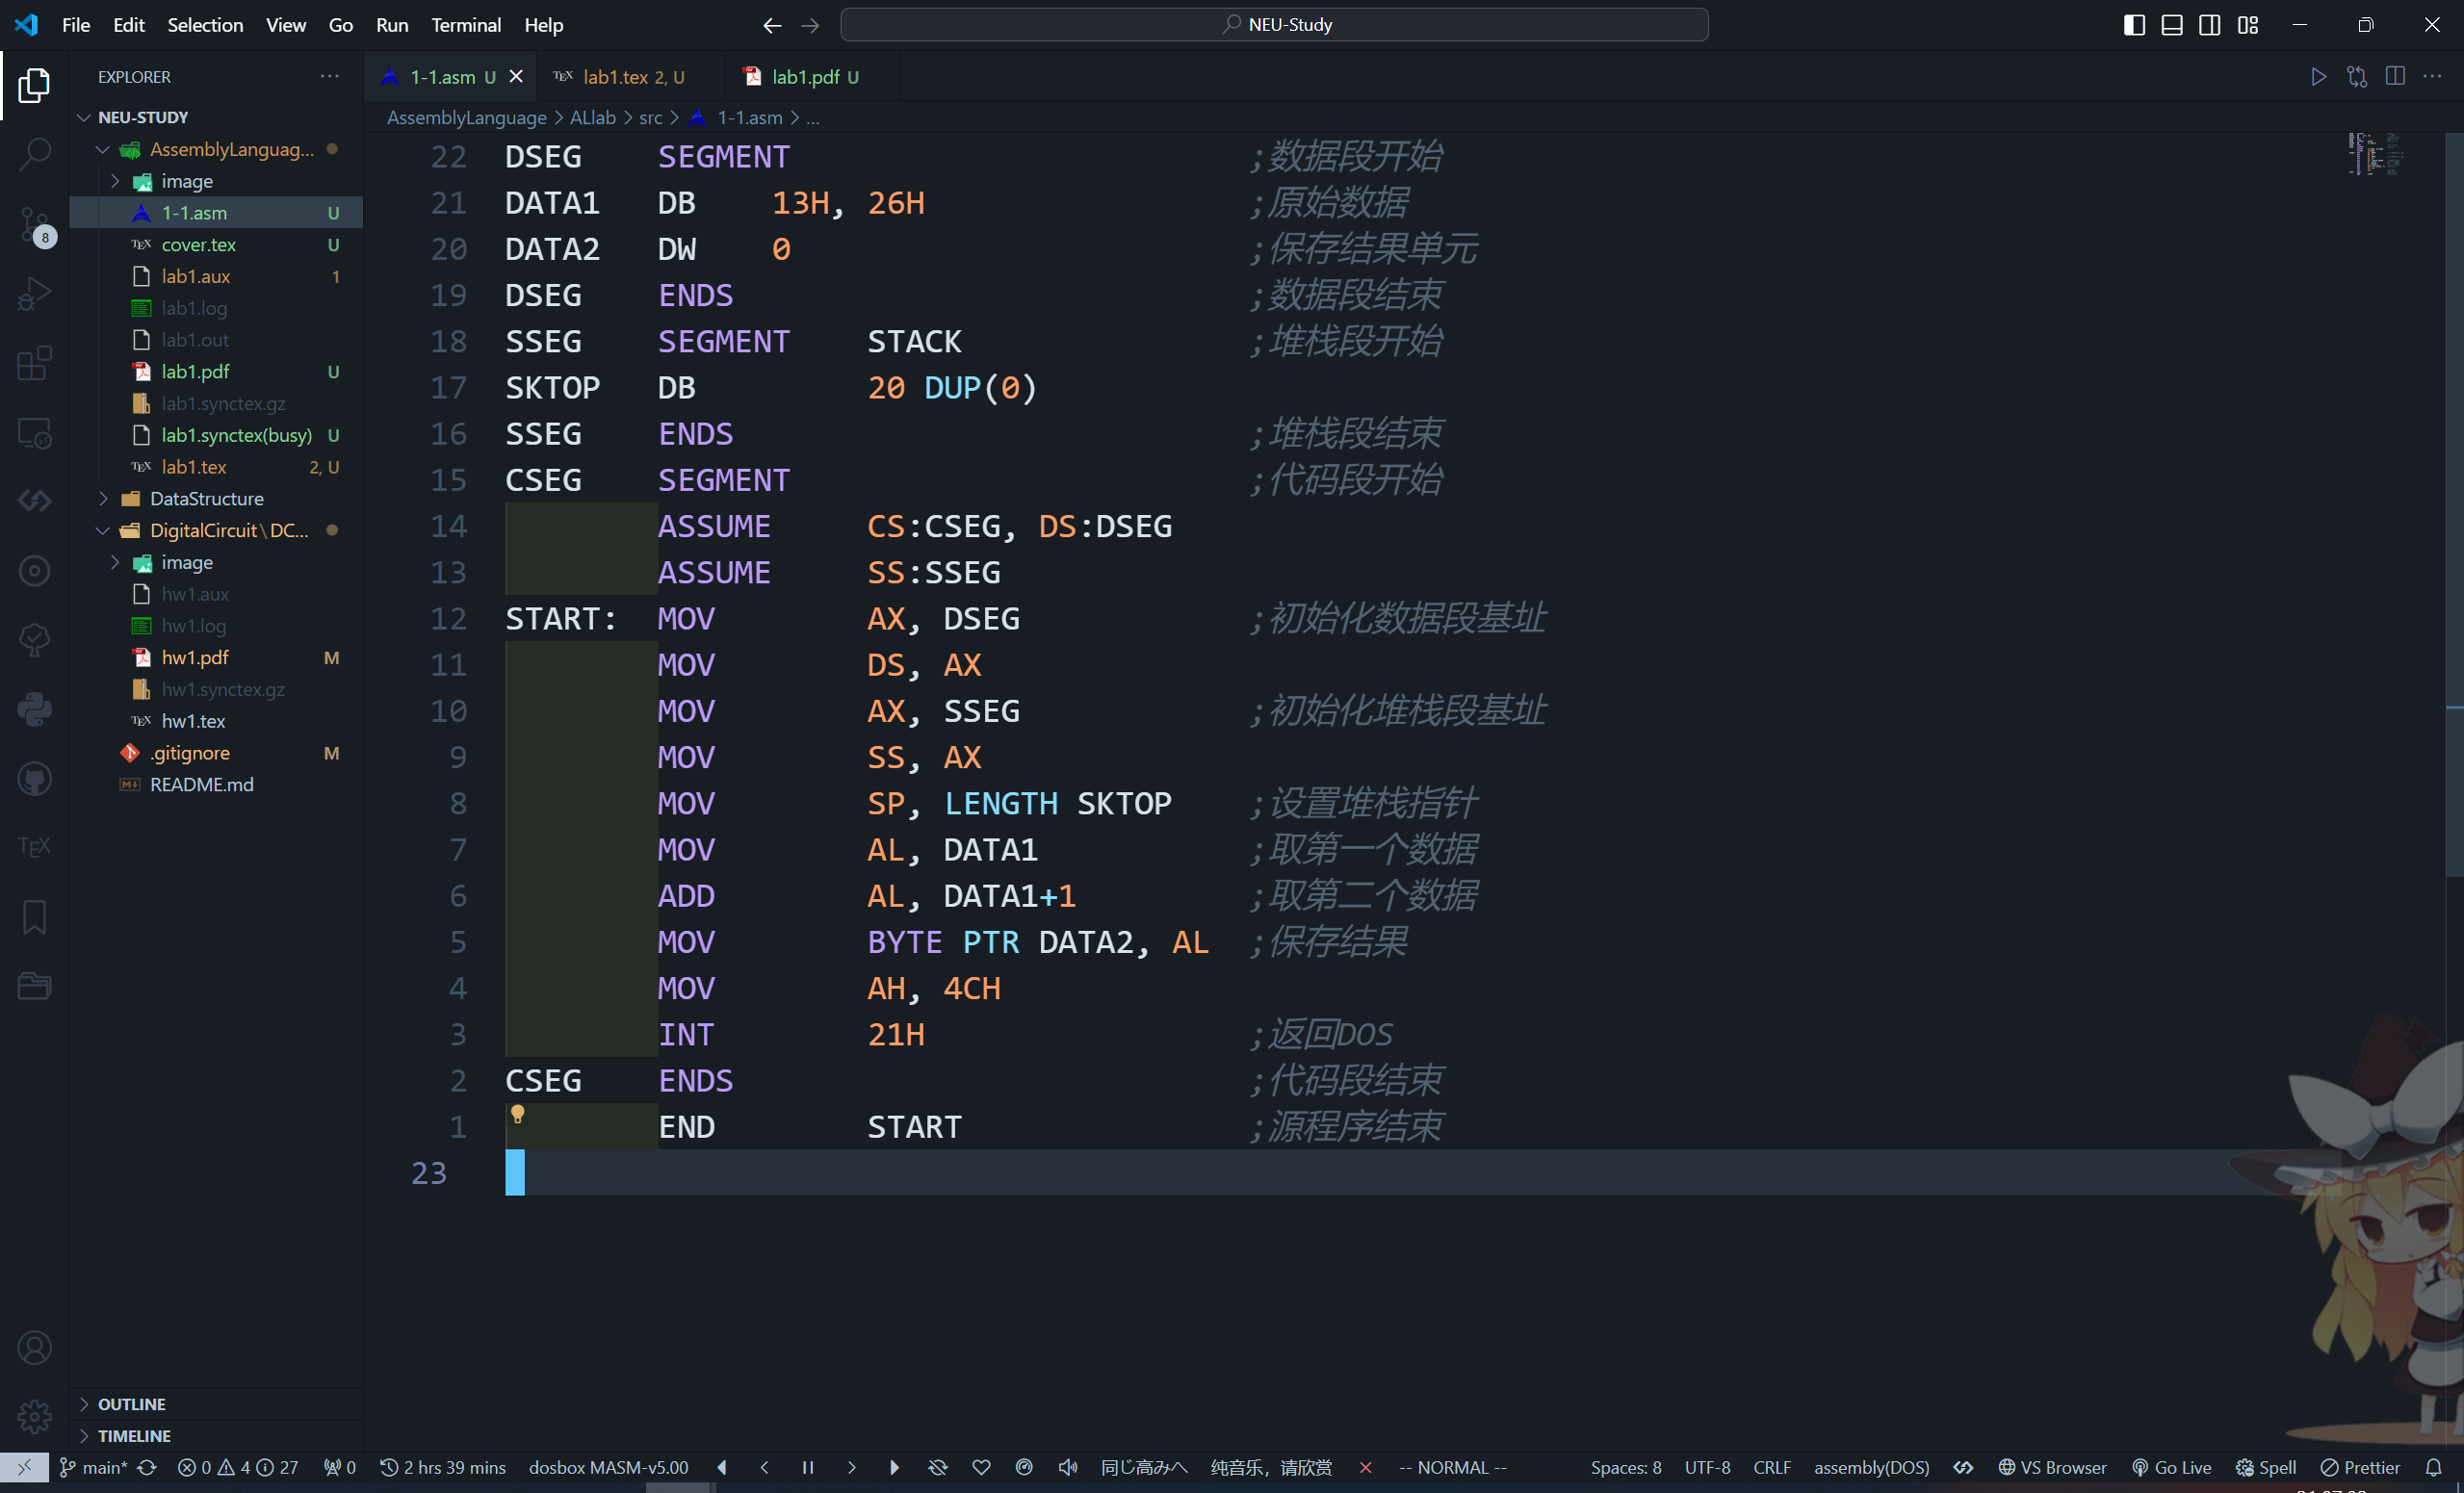
\includegraphics[width=1\textwidth]{image/AL_1.png}\end{center}
        
        汇编、连接源程序如图所示：
        \begin{center}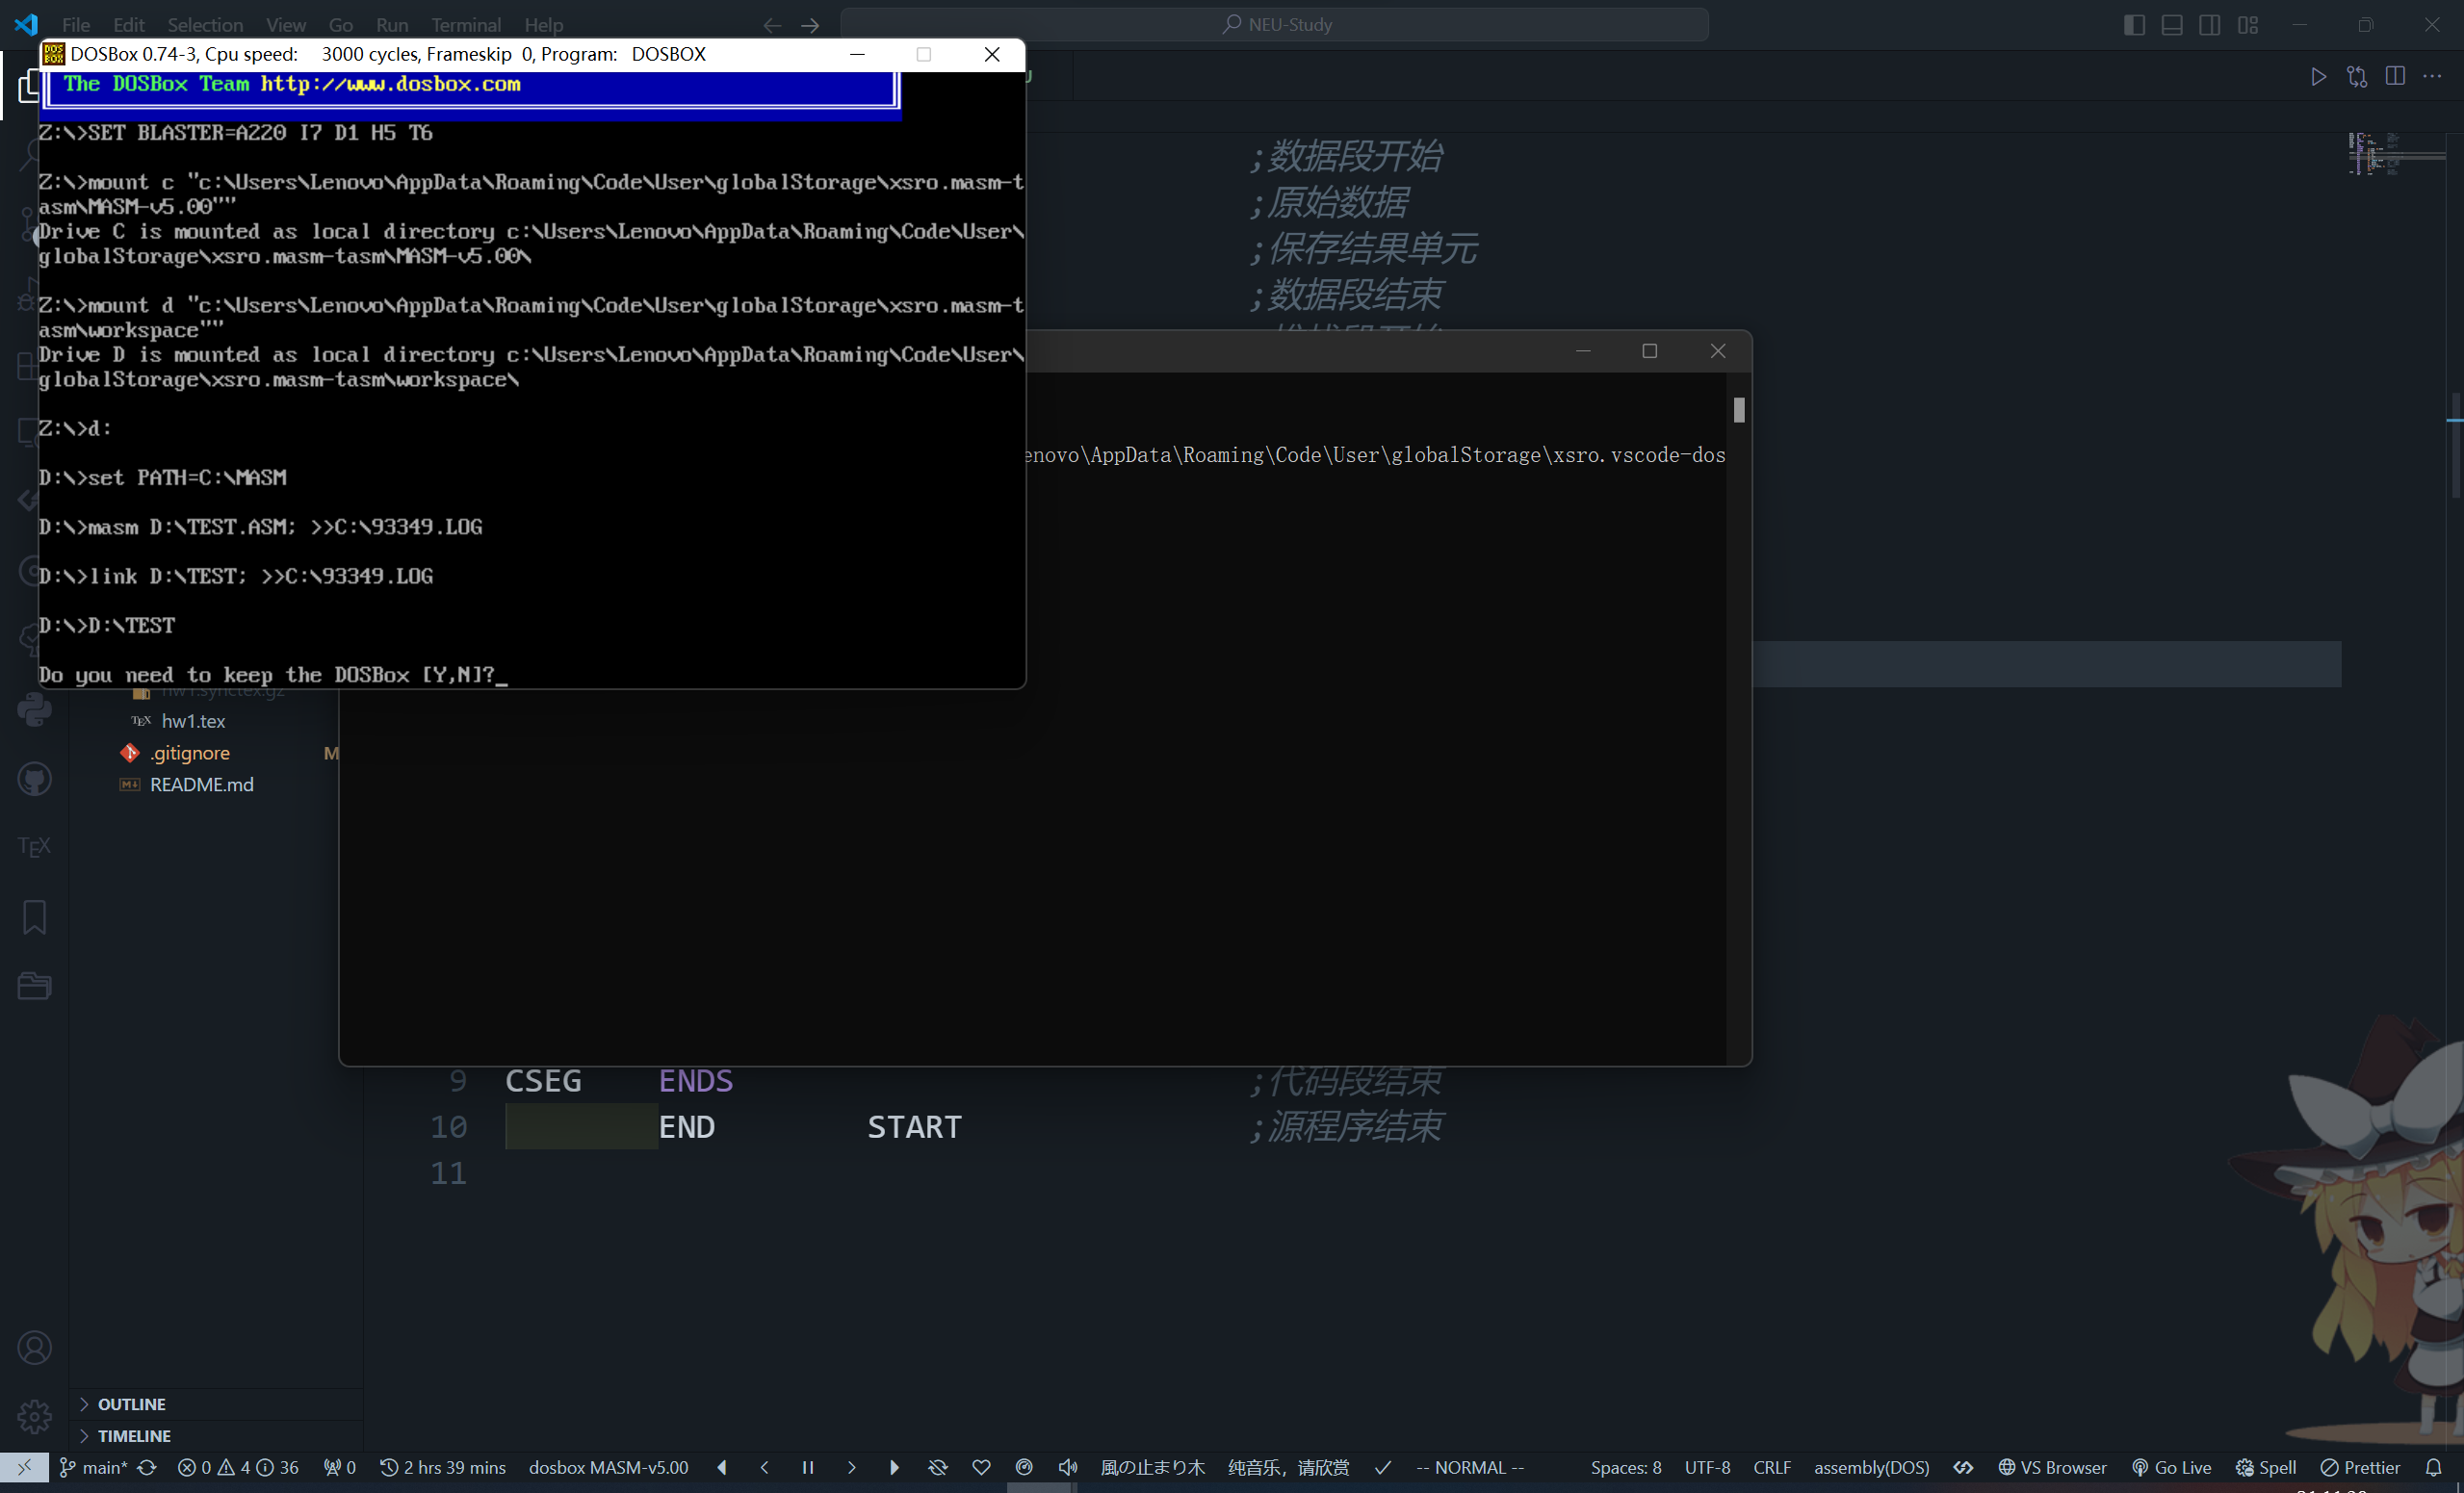
\includegraphics[width=1\textwidth]{image/AL_2.png}\end{center}

        调试源程序如图所示：
        \begin{center}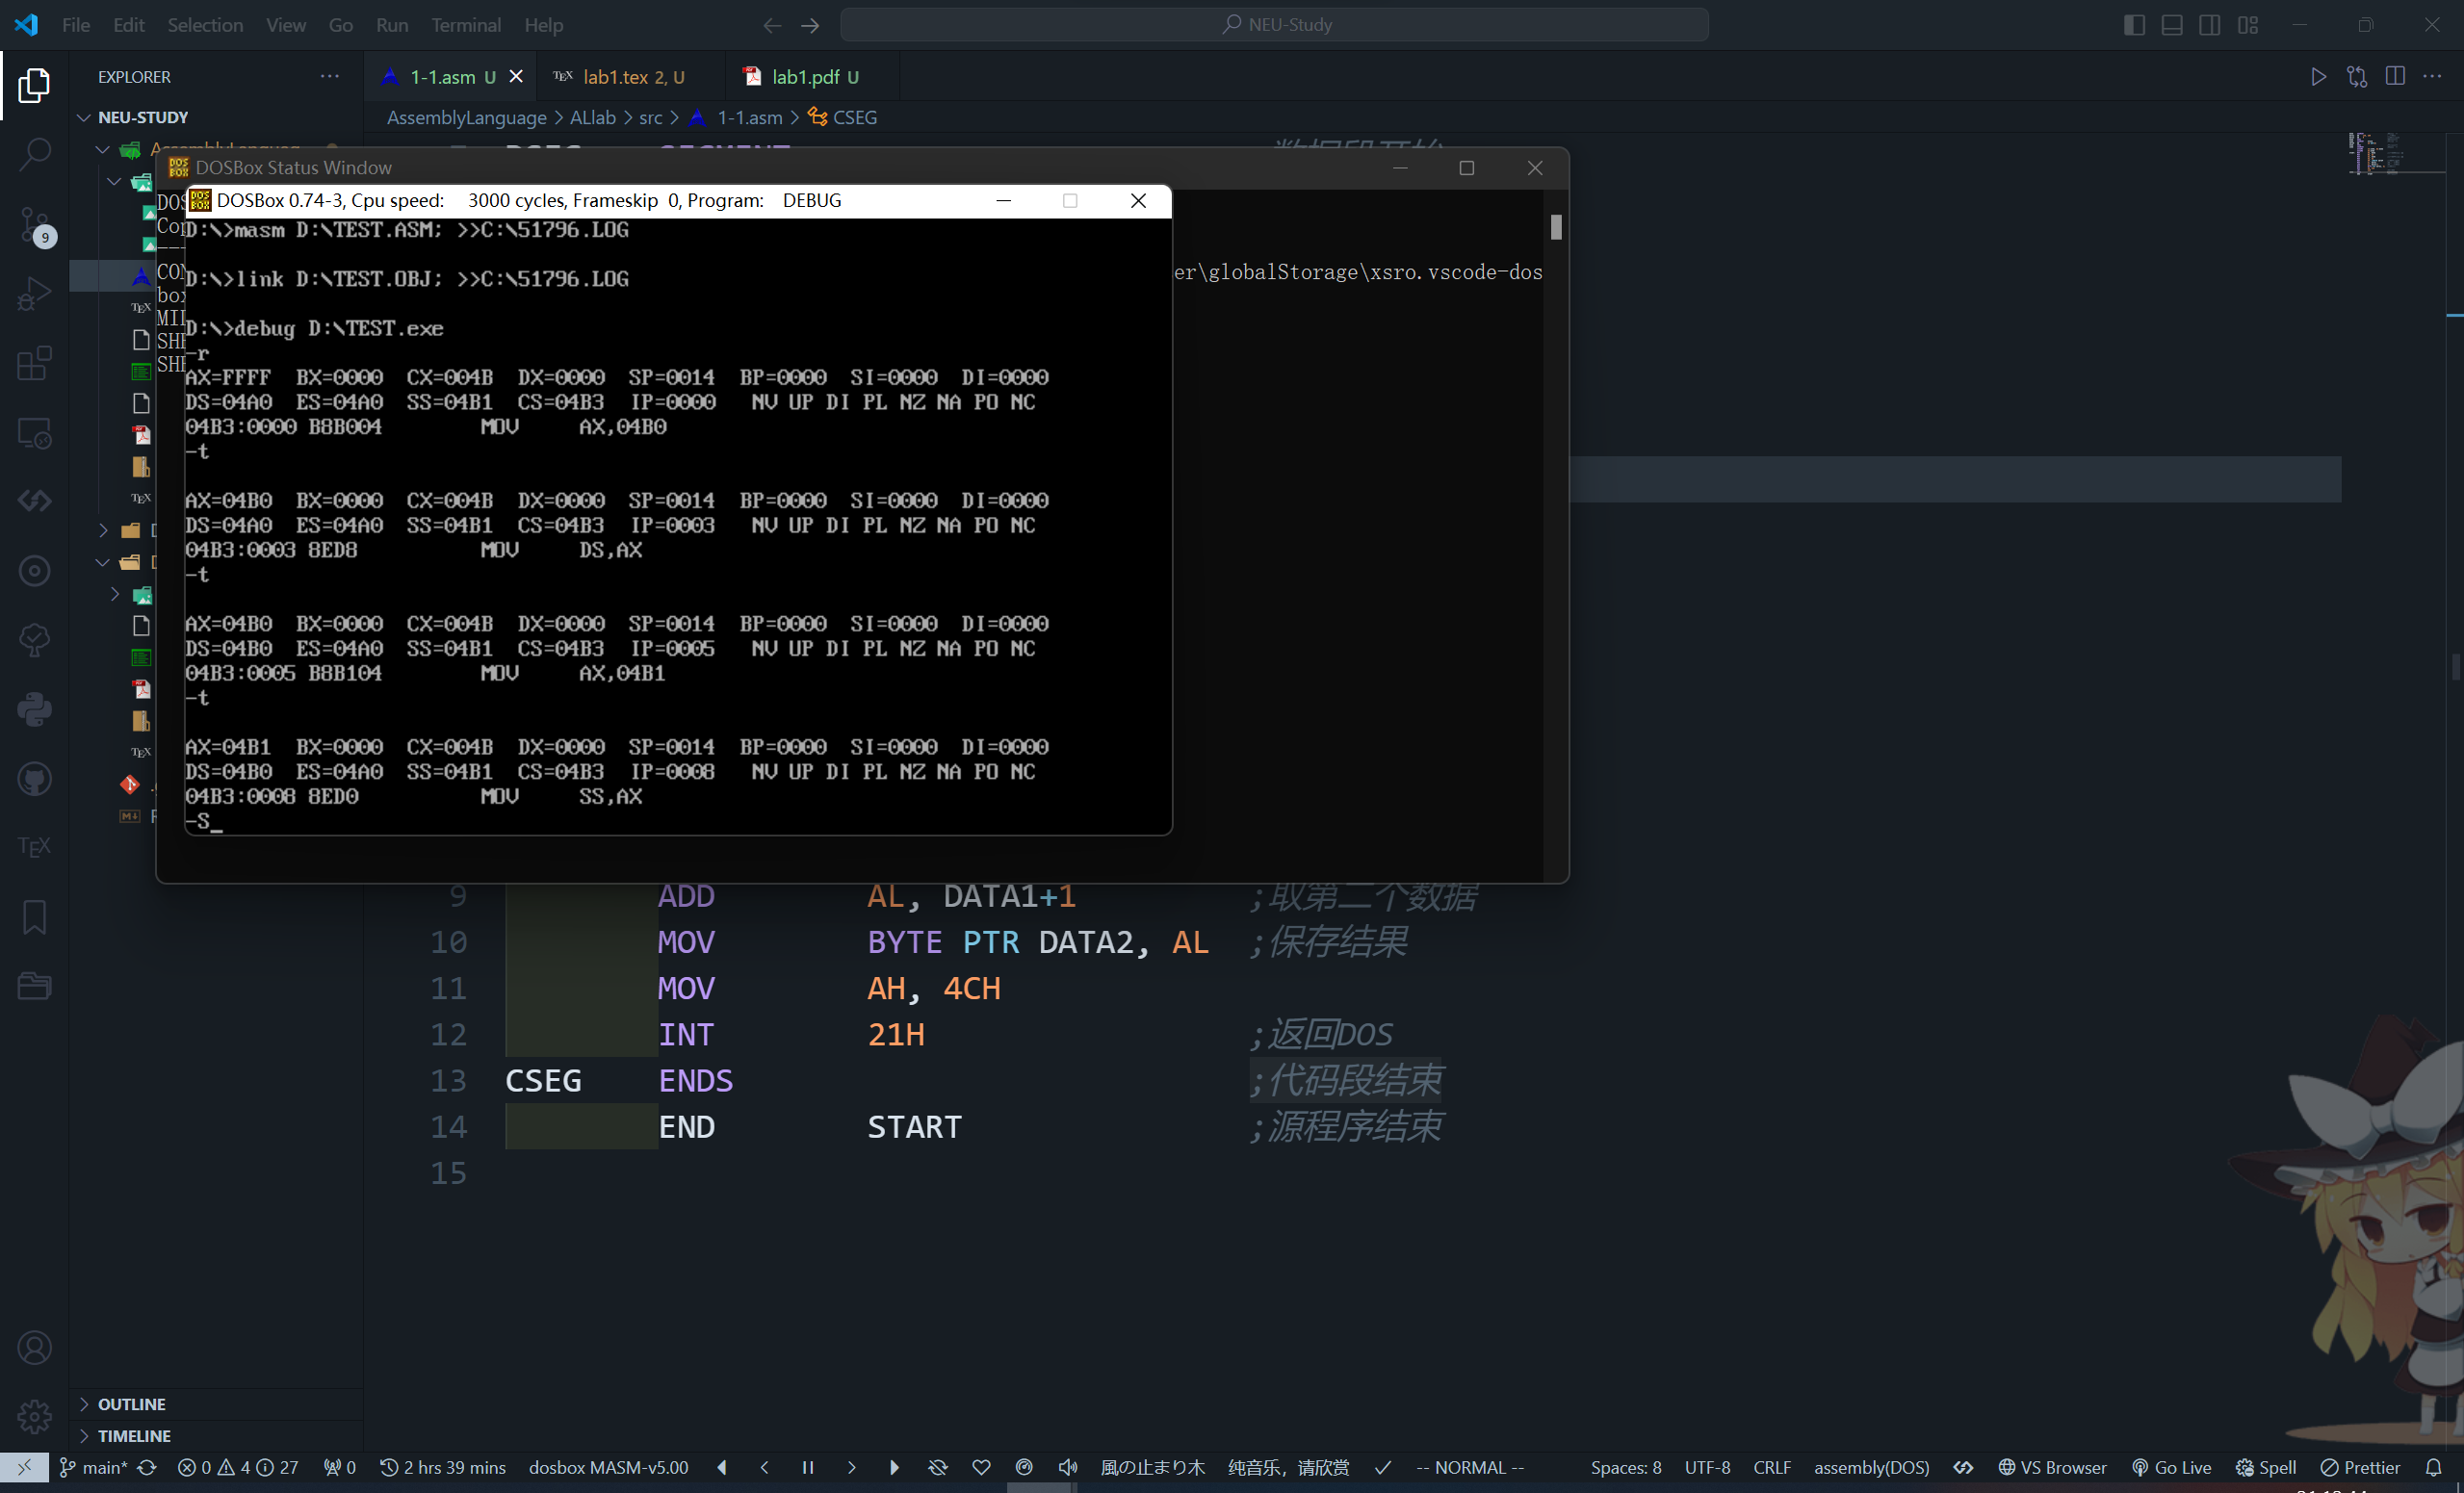
\includegraphics[width=1\textwidth]{image/AL_3.png}\end{center}

    \subsubsection{修改原始数据、执行程序}
        修改原始数据如图所示：
        \begin{center}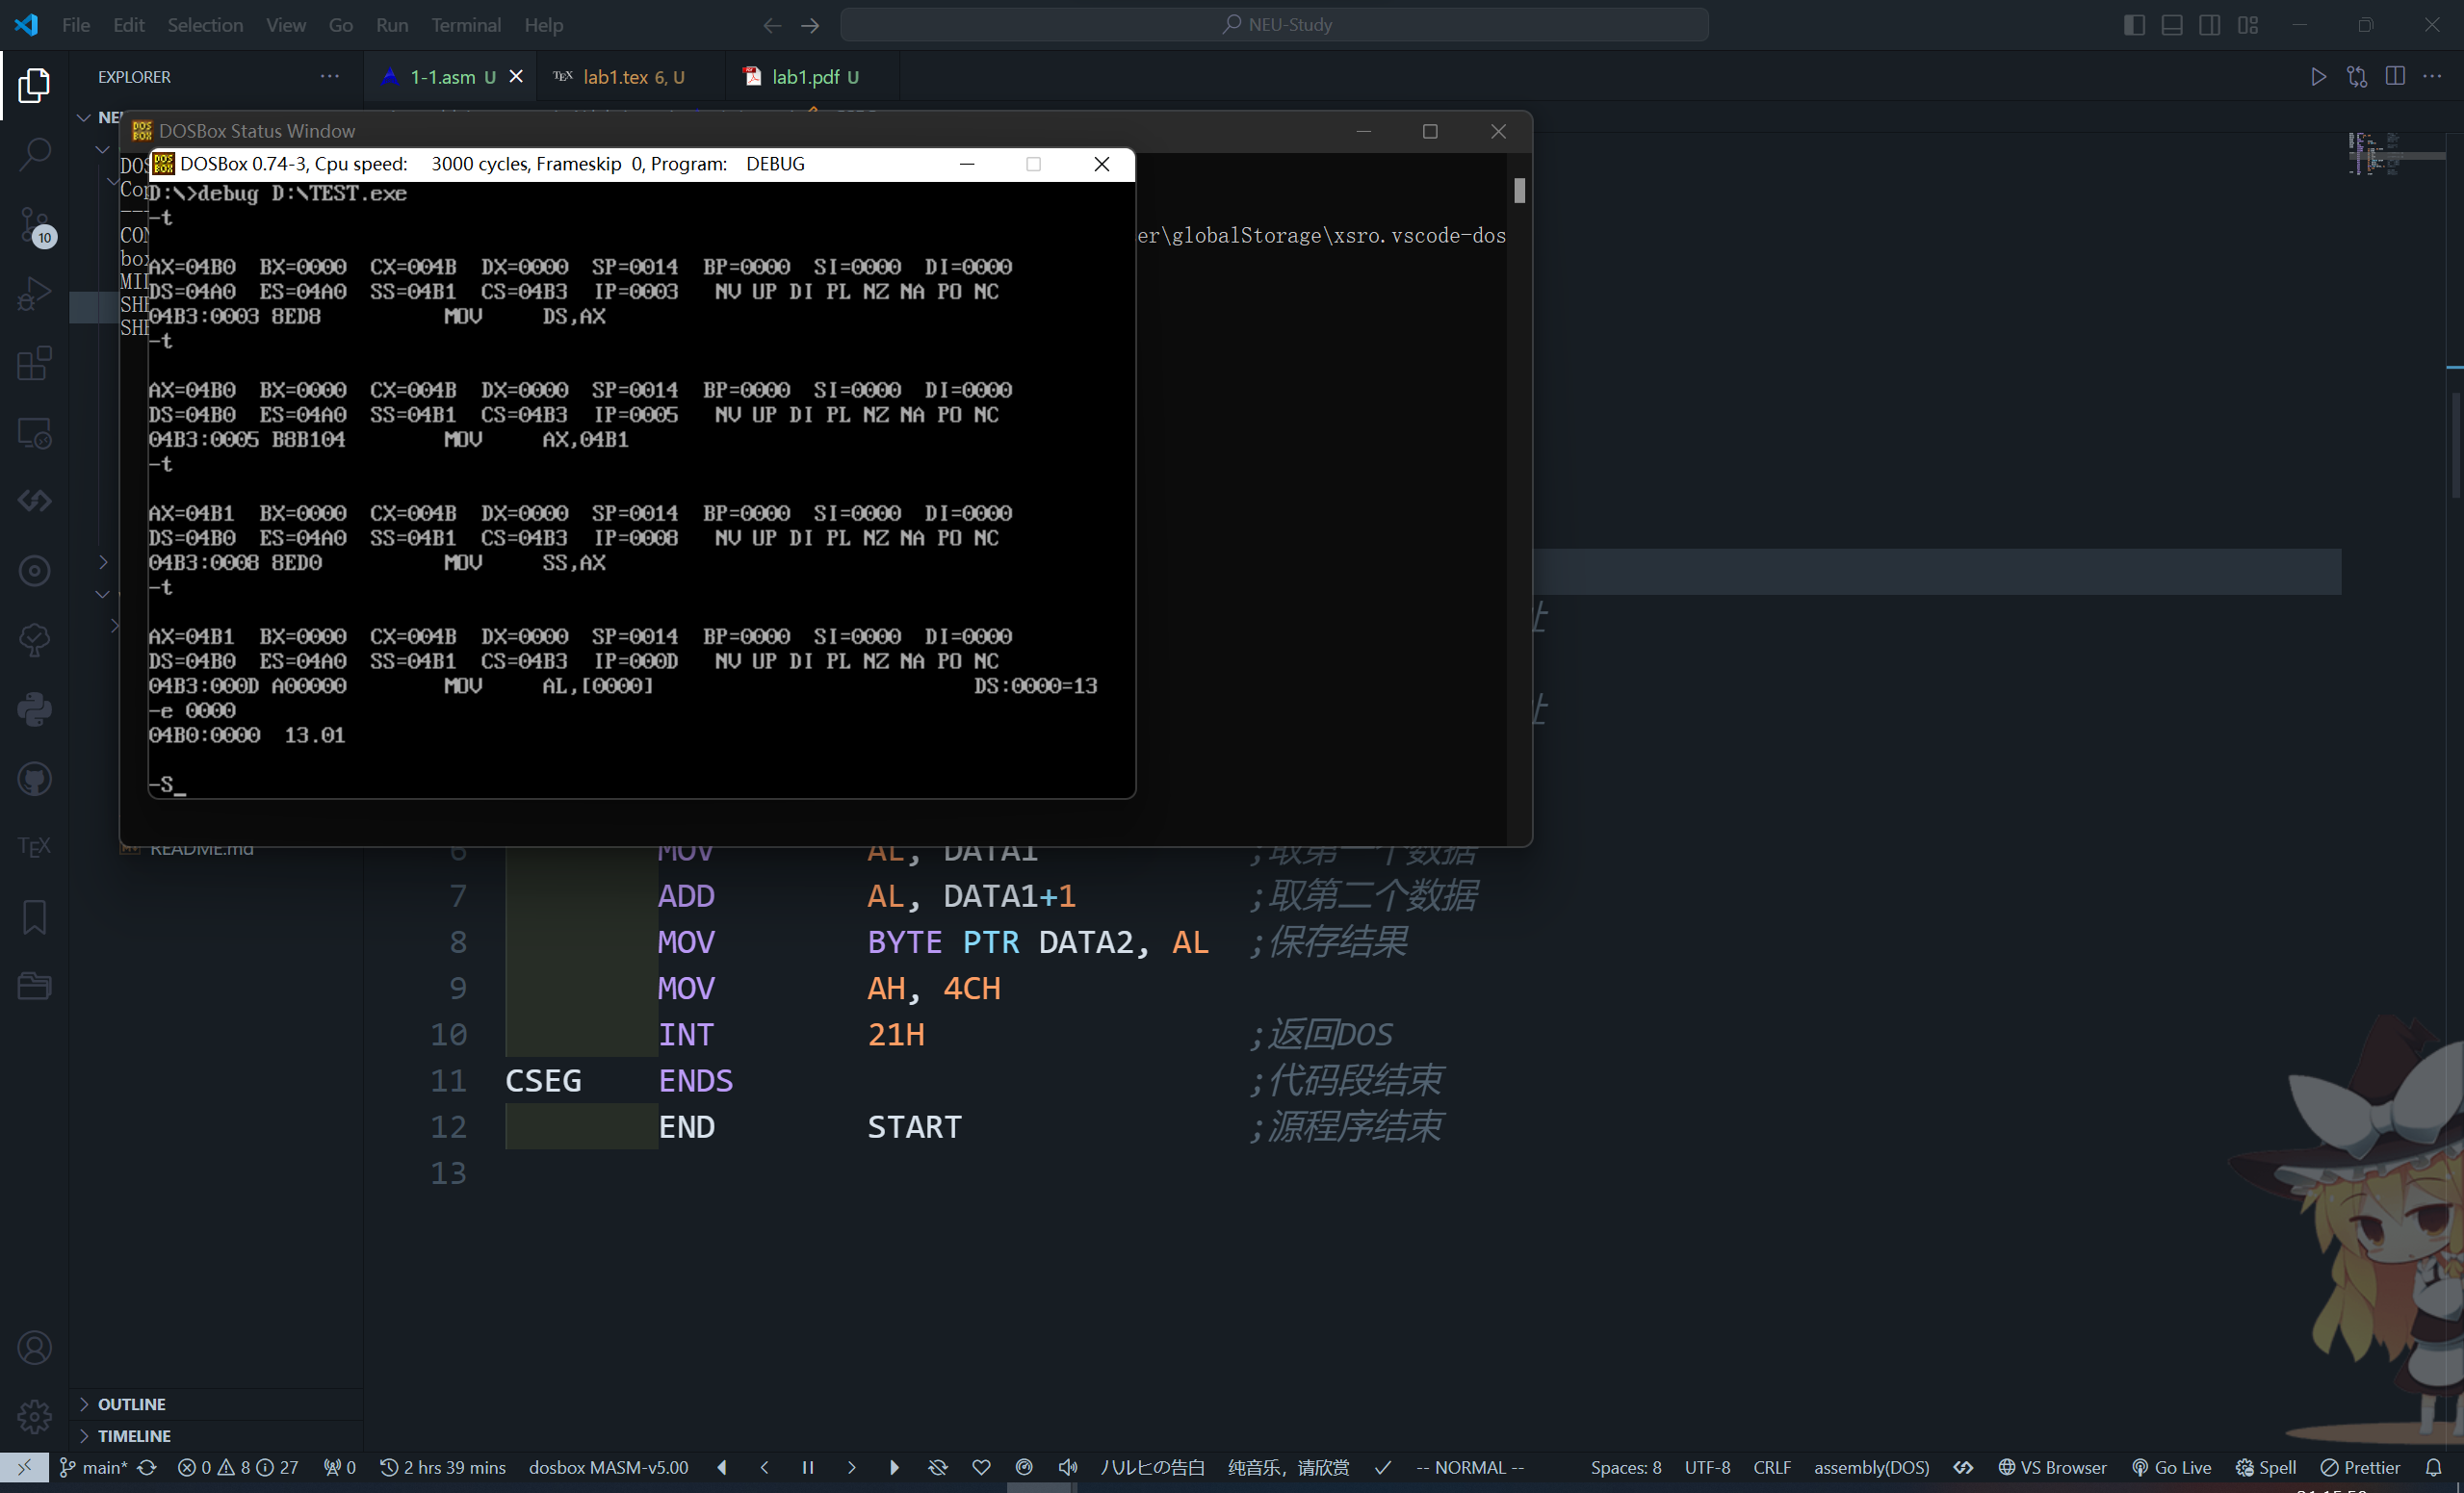
\includegraphics[width=1\textwidth]{image/AL_4.png}\end{center}
        
        用G命令执行程序如图所示：
        \begin{center}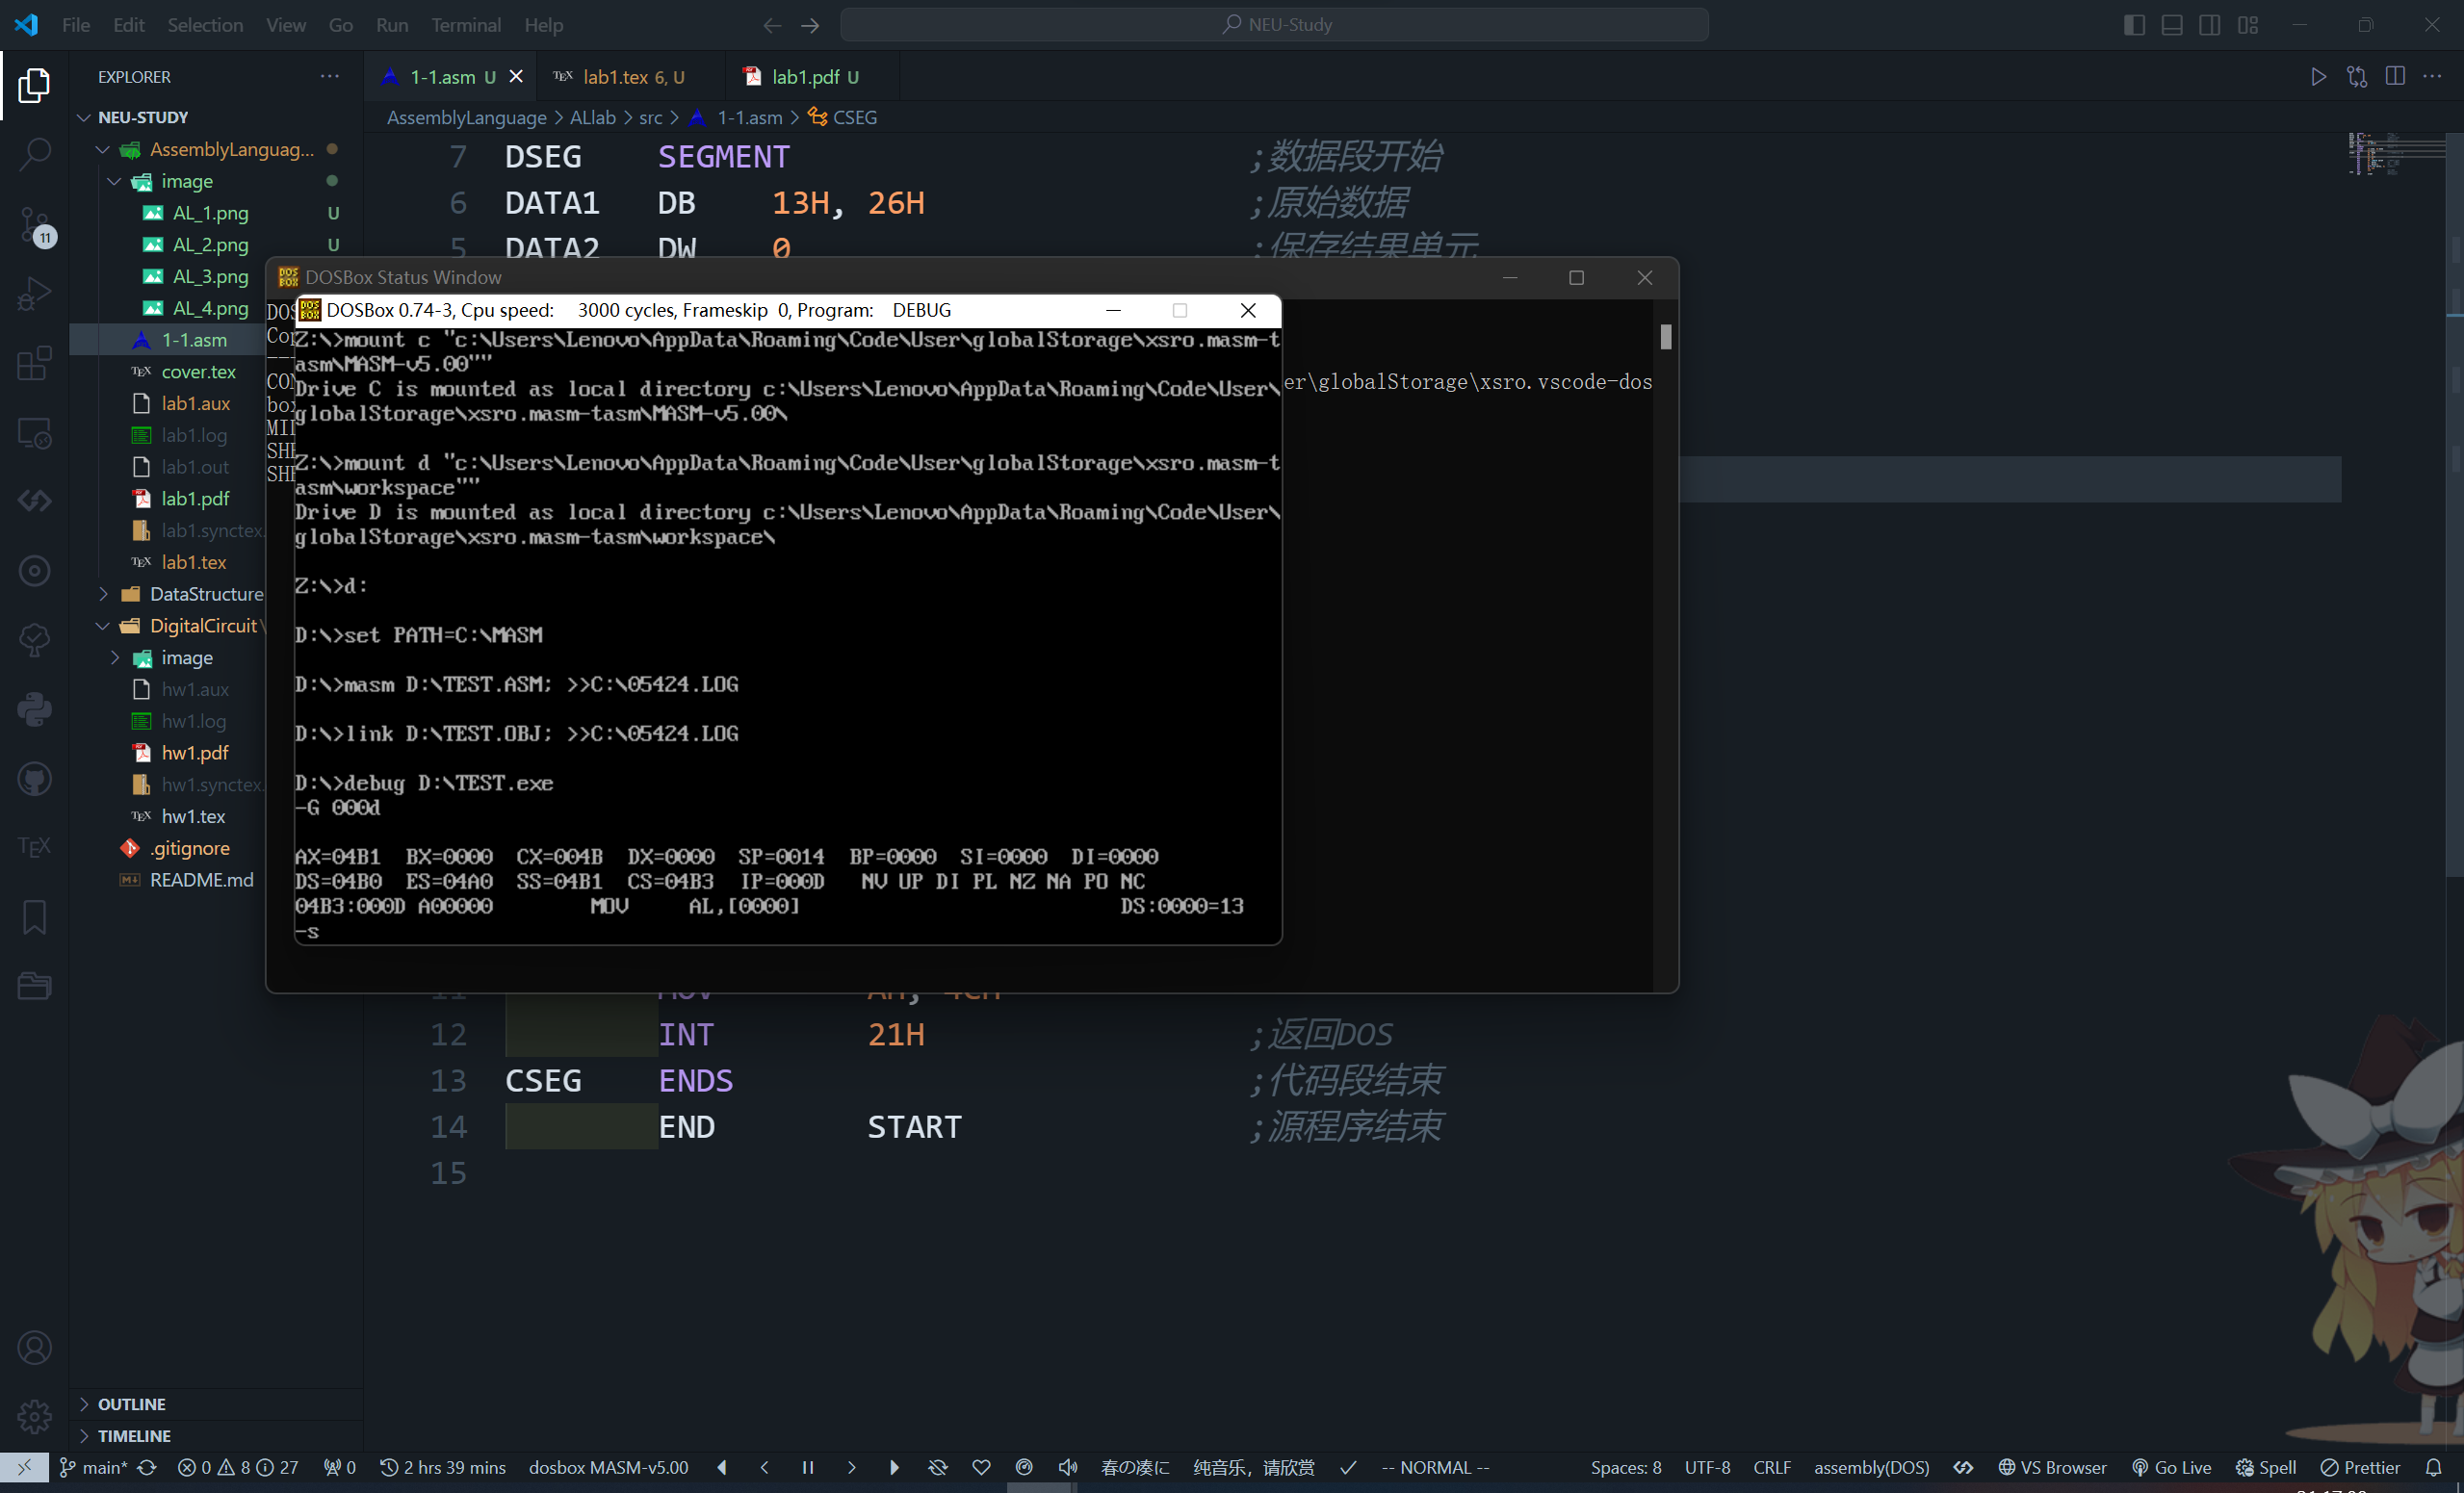
\includegraphics[width=1\textwidth]{image/AL_5.png}\end{center}

    \subsubsection{修改程序}
        用DEBUG中的A命令修改程序如图所示：
        \begin{center}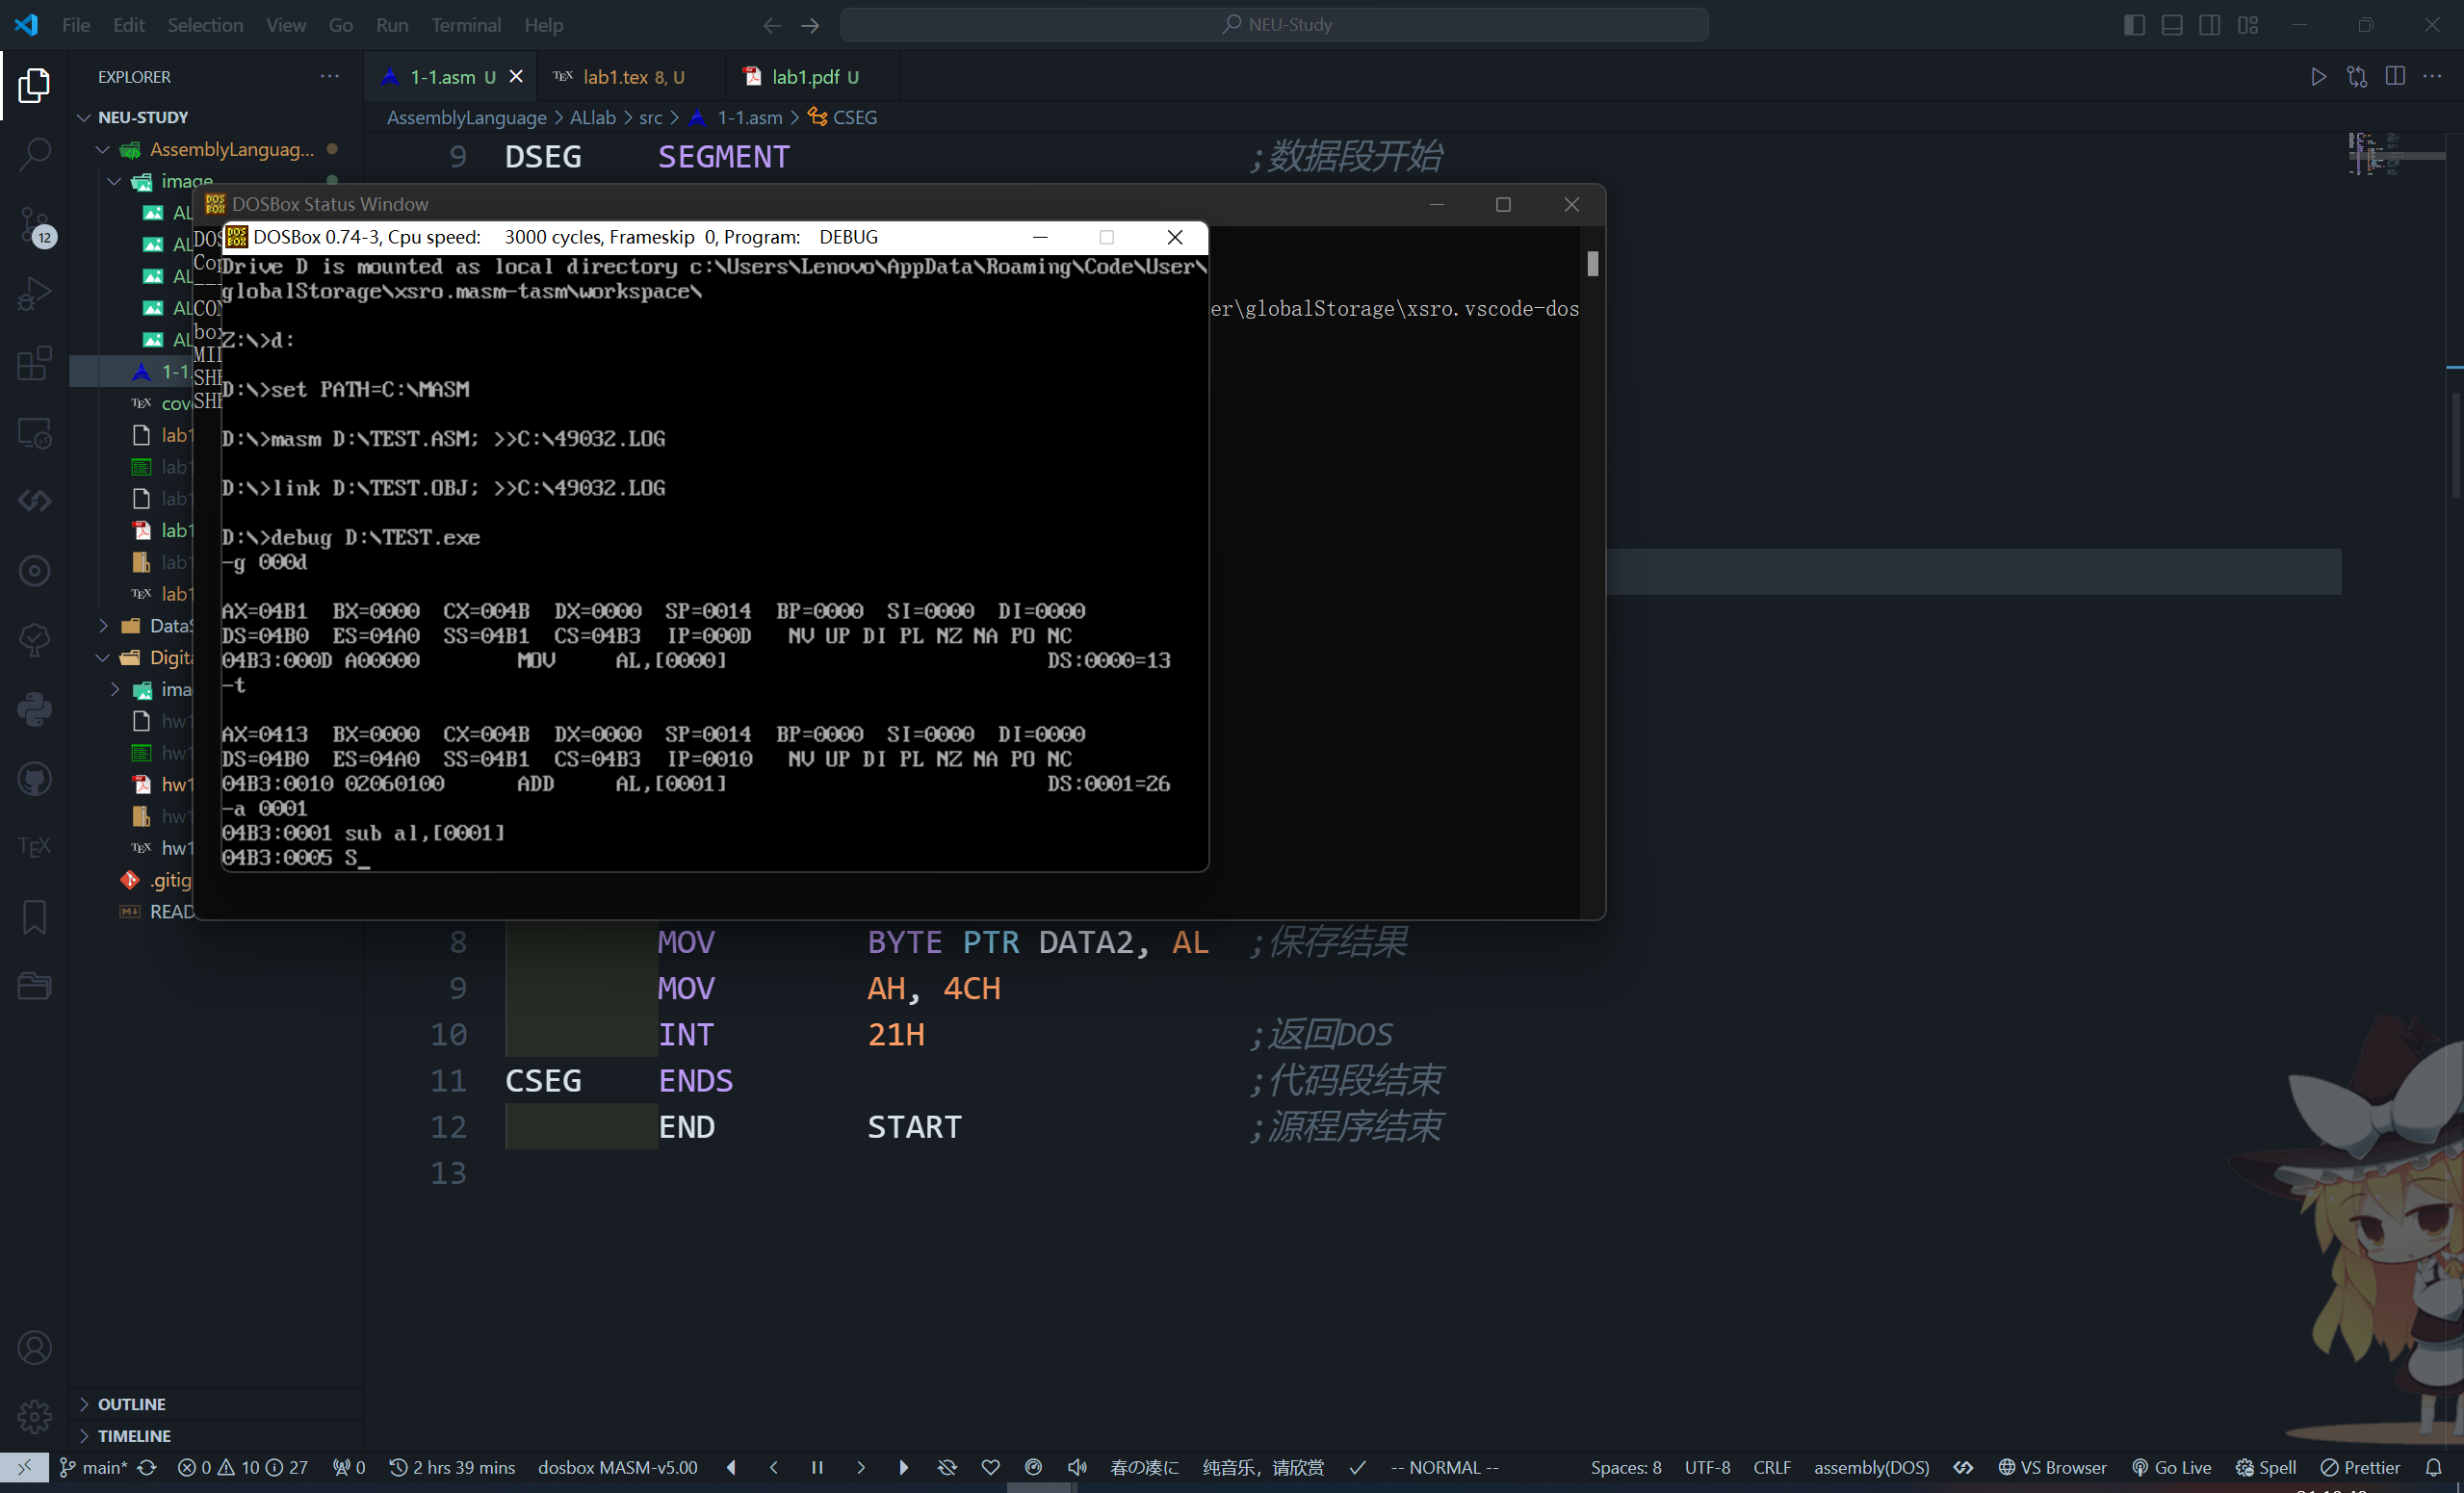
\includegraphics[width=1\textwidth]{image/AL_6.png}\end{center}


    \subsection{题目二}
    任选一组有代表性意义的数据（要求有正数、负数、ASCII码常数），分别用DB、DW和DD加以定义如图所示：
    \begin{center}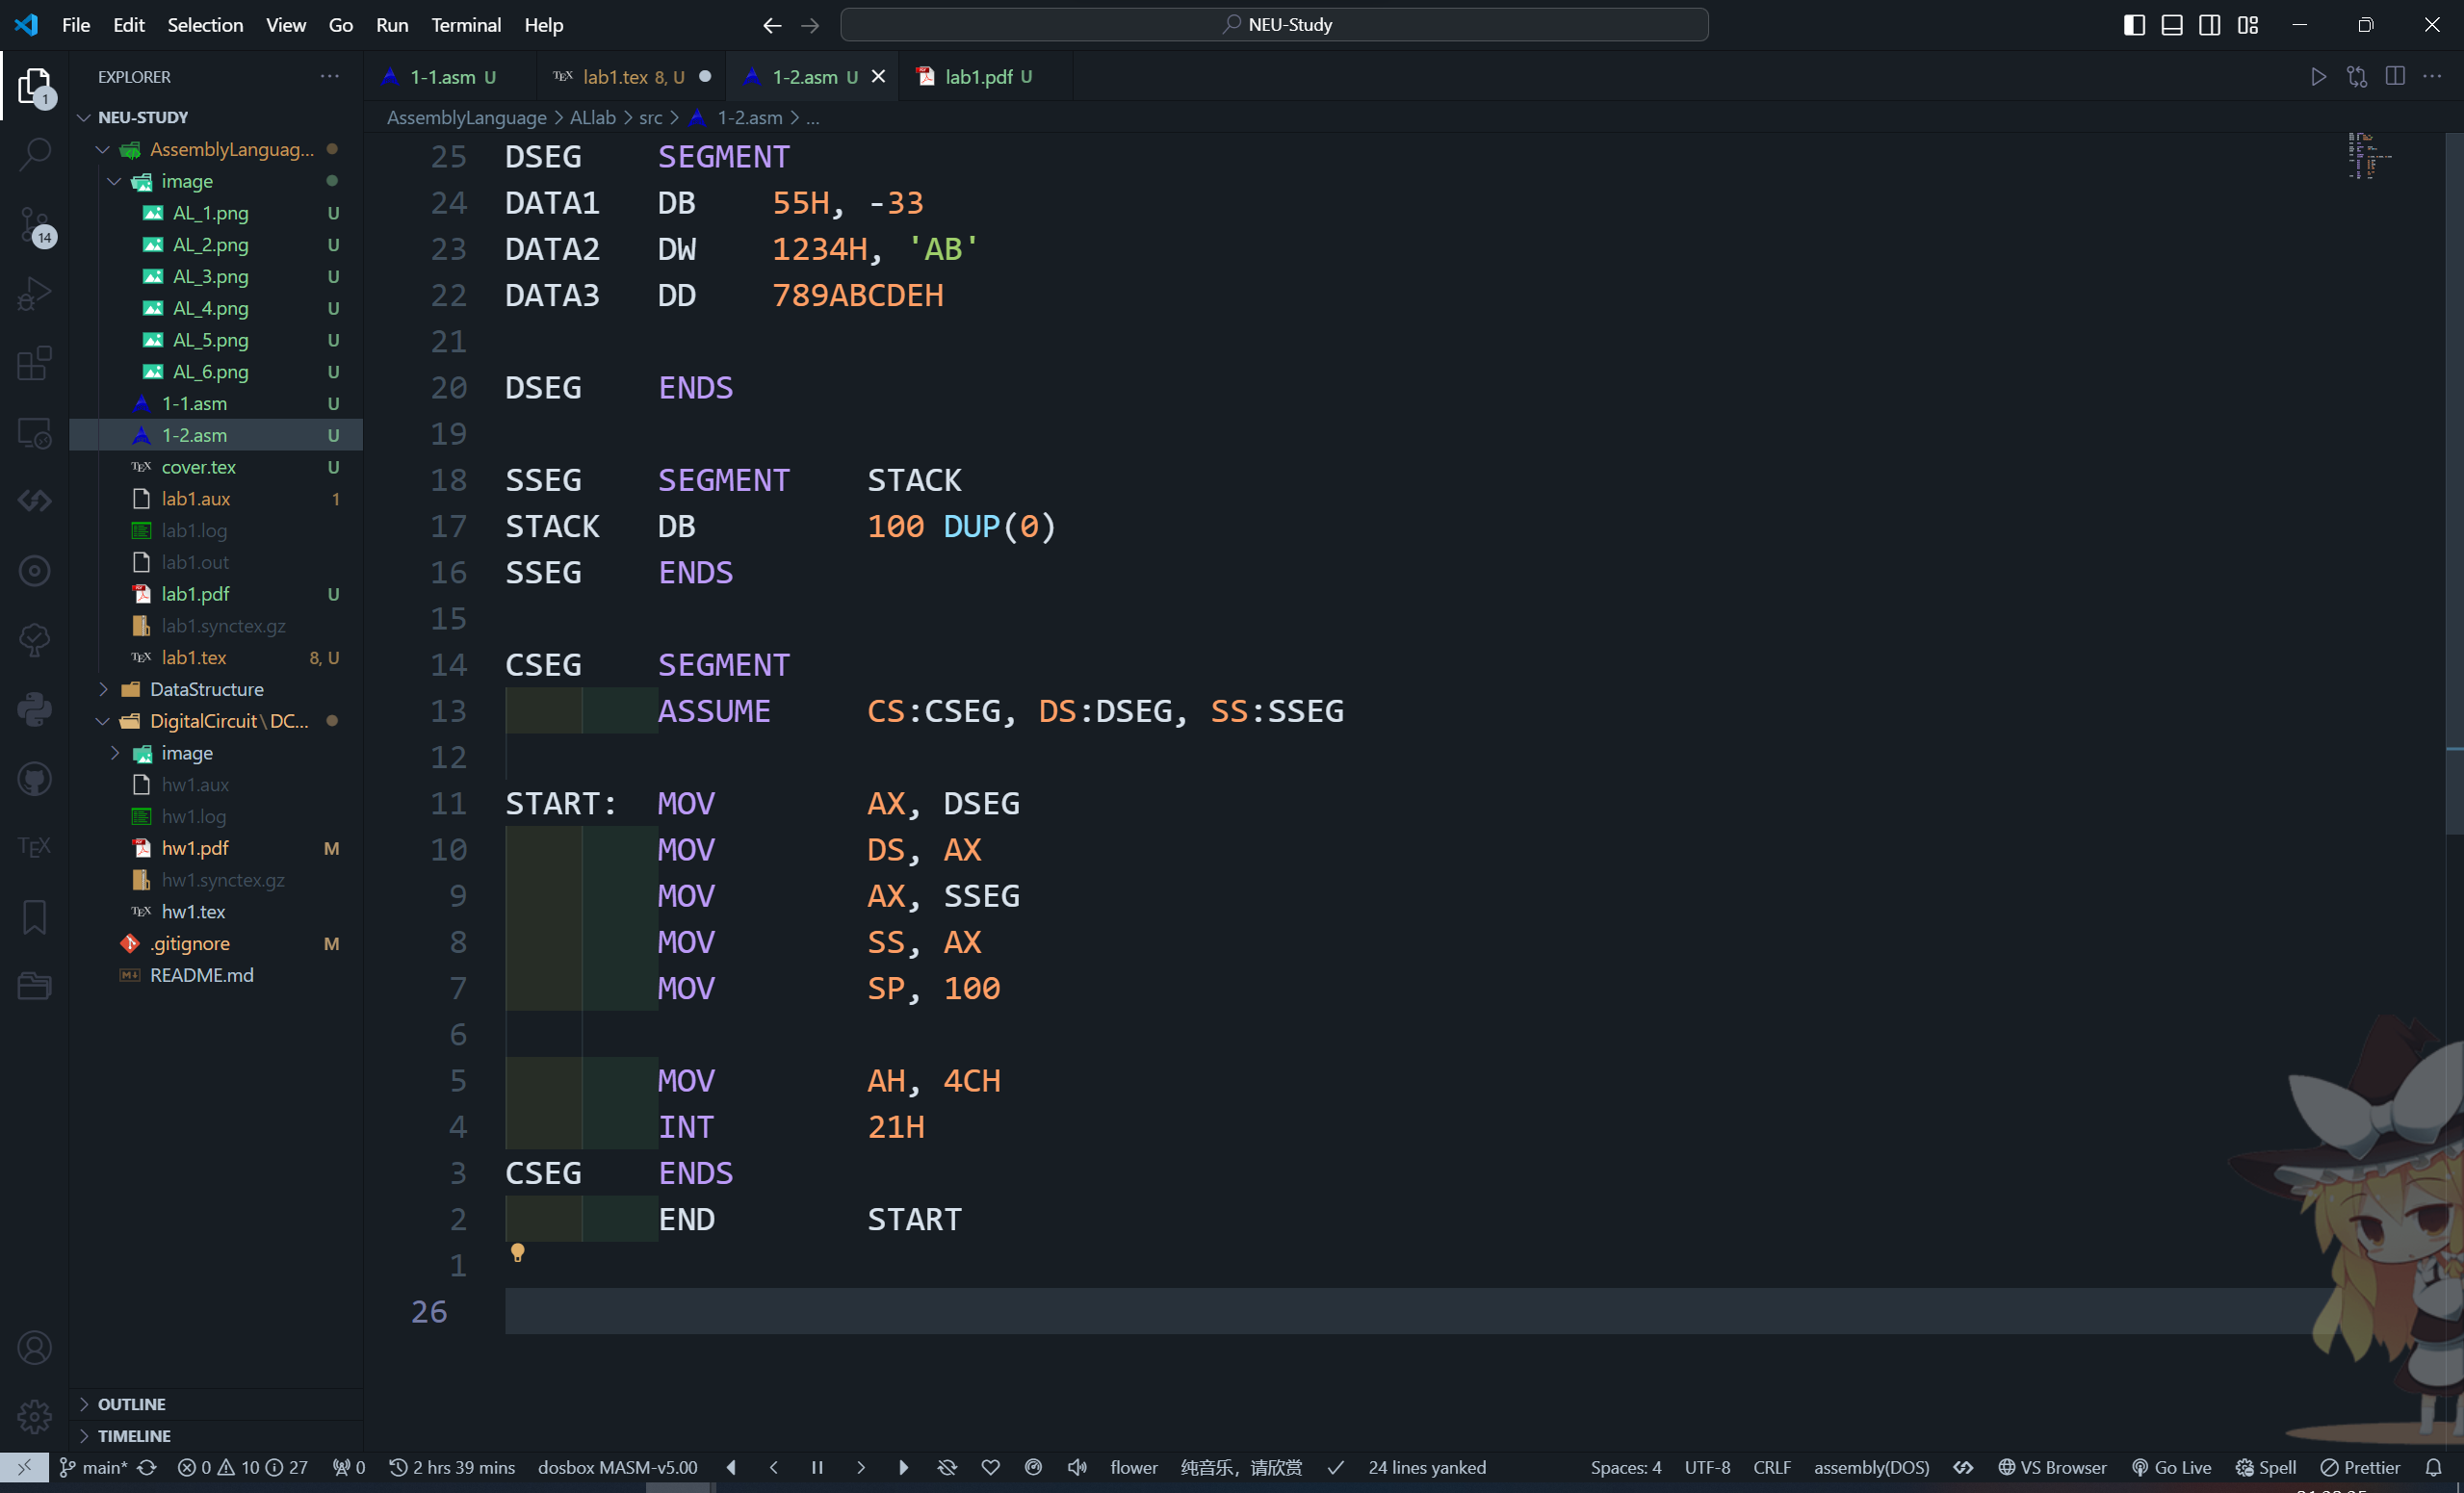
\includegraphics[width=1\textwidth]{image/AL_7.png}\end{center}
    
    
    观察汇编后在机器内部的存储情况如图所示：
    \begin{center}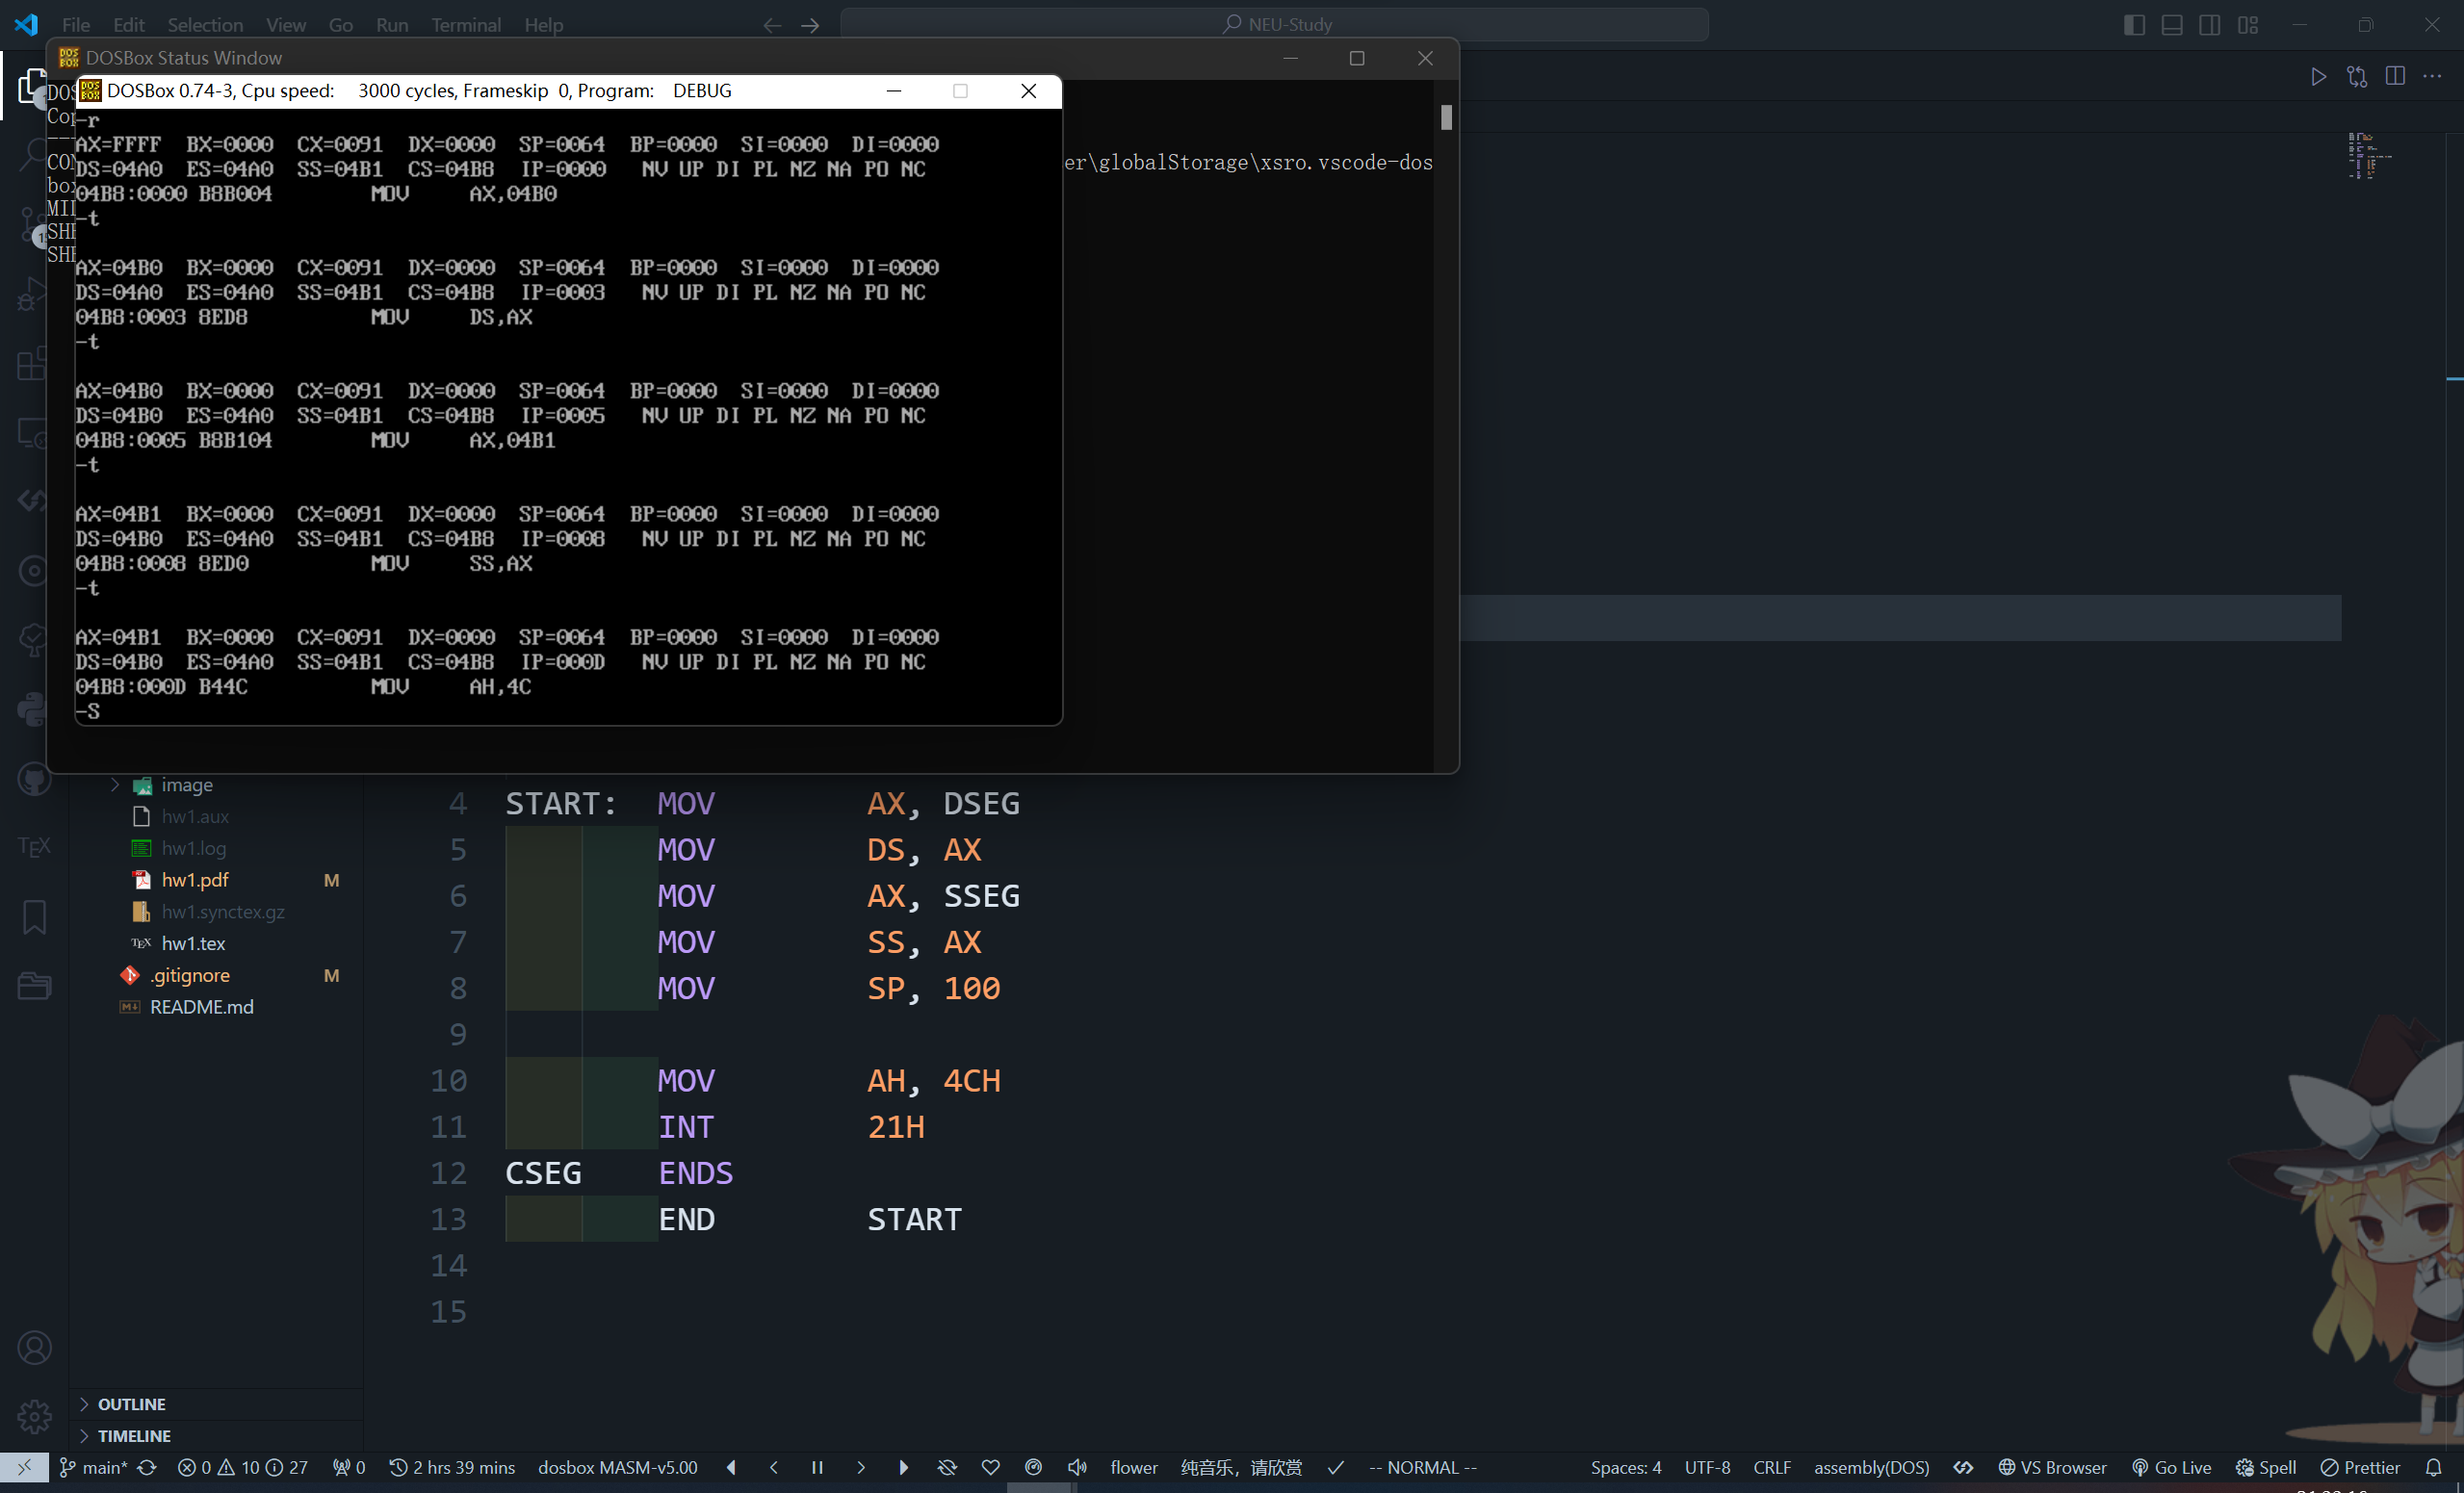
\includegraphics[width=1\textwidth]{image/AL_8.png}\end{center}

\section{心得体会}
    通过本次汇编语言程序设计的实验，我对汇编语言有了更加深刻的理解。
    在实验中，我不仅学会了如何编写、编辑、汇编和调试汇编语言程序，而且还学到了如何使用DEBUG工具进行有效的程序调试。

    一个主要的挑战是在使用DEBUG工具时遇到的问题。
    最初，我发现使用DEBUG命令来跟踪程序执行过程相当困难，尤其是在定位错误和理解程序流程方面。
    通过反复练习和参考教材，我逐渐熟悉了各种命令，如U（Unassemble）、D（Dump）等，并能够更有效地调试我的程序。

    实验中的数据定义和内存分配部分也是一个学习重点。
    通过定义不同类型的数据（如正数、负数、ASCII码常数）并观察它们在内存中的分布，我对汇编语言的数据处理有了更全面的了解。我学会了如何使用DB、DW和DD指令，并理解了它们在内存分配上的差异。

    这次实验不仅增强了我的汇编语言编程技能，还提升了我的逻辑思维能力和问题解决能力。
    通过实际操作，我更加清楚地理解了理论知识，并能够将这些知识应用于实际问题中。
    我期待在未来的学习中继续探索更多关于汇编语言的深入知识。


\begin{flushright}\begin{tabular}{rl}
    姓名: & 李俊洁\\
    班级: & 计算机2204 \\
    学号: & 20225443 \\
    课程: & 汇编语言程序设计 \\
    日期: & March 27, 2024 \\
    制作: & \LaTeX \\
    & 感谢您的批阅！
\end{tabular}\end{flushright}
\end{document}
